% Copyright (c) 2014,2016 Casper Ti. Vector
% Public domain.

\specialchap{引言}
图是一种表达能力丰富的数据结构,一般用G = (V, E)表示一个图,其中V是图中的点集,E是图中的边集。如果图中的边是有方向的,则称该图为有向图。在有向图中,如果两条边具有相同的起点和终点,则称这样的边为重边(multi-edge)。属性图\supercite{property_graph}是一种带重边的有向图,图中的每个元素(点/边)可以拥有任意数量的属性值。特别地,每个元素都有一个label属性,标识该元素的类别。
实际应用中,有些属性图会含有大量重边。比如在电信行业的通话关系图中,两人之间可以发生多次通话关系;又比如金融行业的交易关系图中,两人之间可以发生多次交易关系。更复杂的,在刑侦应用中,整个情报系统获得的信息融合成一个知识图谱\supercite{knowledge_graph},其中的实体和关系类型丰富多样。比如实体类别有人、汽车、公司等,实体间的关系有亲属关系、共同出行关系、通话关系等。有的关系是可以多次重复的,频次可能成百上千,这使得两个实体间不仅有多种label(即多种关系)的边,还包含大量重边。图\ref{fig:property_graph}是属性图在刑侦场景中的一个简单示例,显示了类型为人的结点以及通话关系和共同出行关系。其中共同出行关系是双向的,因此在图中以无向边表示。刑侦场景中的典型查询包括:从一个人出发查询与其相关的所有人(邻域点集查询)、查询两个人在几跳内是否有关系(路径查询)、查询两人之间的所有关系(两点间边集查询)等。

\begin{figure}[htbp]
\centering
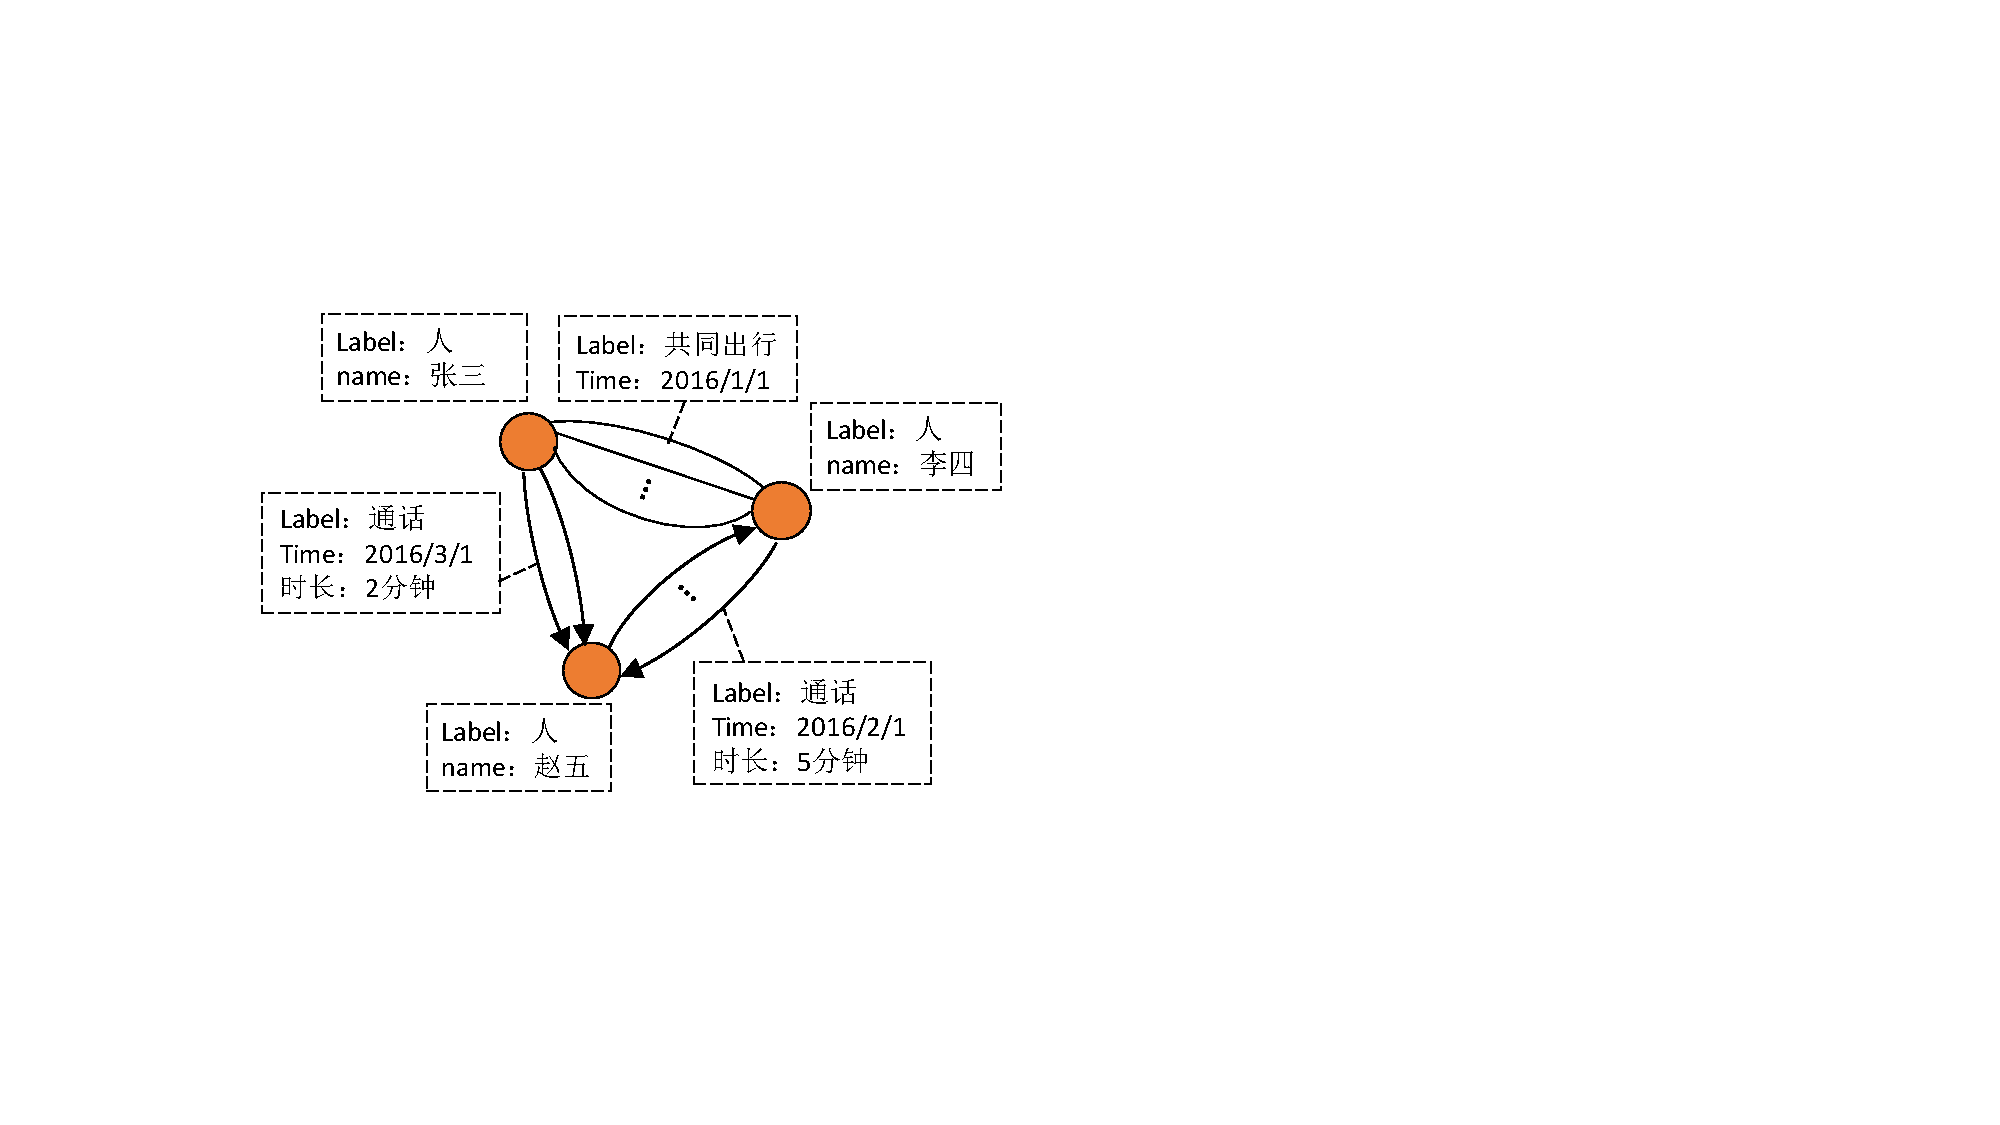
\includegraphics[width=100mm]{fig/property_graph.pdf}
\caption{属性图示例}
\label{fig:property_graph}
\end{figure}

传统解决方案将数据存储在关系型数据库中,如将所有通话数据存储在通话关系表中。关系型数据库能胜任图数据的存储,也能方便地检索元素的内容,但在图结构相关的查询上表现欠佳。比如两跳邻域查询,锁定一个嫌疑人后,要查看其两跳范围内的子图信息。为得到第二跳的邻域结点,需要对各种关系表做昂贵的JOIN操作。图数据库由于其以图的形式存储数据,在图的拓扑结构查询中具有更优异的性能。因此当应用场景中图的拓扑结构查询与元素的内容查询同等重要时,图数据库是最佳的选择。明略数据 是一家大数据解决方案提供商,客户群涵盖刑侦、金融、电信等领域。其中SCOPA 是明略数据的重要产品,在海量刑侦数据上构建起一个数据分析挖掘平台,展现给领域专家的是一张属性图,关联了客户原有的所有数据。SCOPA平台即使用图数据库实现其存储核心。
然而,在富含重边的属性图中,图数据库的查询性能不佳。在传统的图应用中,图中的边一般是稀疏的。如一些公开的图数据集 中,边集的大小约为点集大小的十几倍。但在富含重边的应用场景中,边集大小可能为点集的上万倍。图数据库以邻接表的方式存储图,表中的每一项存储一条边。这使得查询邻接点集时,需要遍历整个邻接表中的所有边。当图中含有大量重边时,邻接表规模巨大,这种数据组织方式导致邻域查询性能严重受损。而邻域查询是大部分图查询的基础,如多跳邻域查询、路径查询、局部聚集系数查询(计算)等,这些查询往往由嵌套的邻域查询实现,随着邻域深度的增加,这种性能受损将被指数级放大。
一种简化重边的建模方式是,将所有同label的重边合并为一条边来表示,边上存储这些重边的所有信息,这样两个实体间的重边数能降低为边的label种类数。然而,将多条重边的数据合并在一条边中存储,会使边的单位数据量骤增,图中的数据粒度过大,同时降低了单条重边的检索和插入效率,每次操作都要先读取相关的所有重边数据,再在其中做查询或插入操作。因此,处理大量重边是一个不可避免的需求。
在许多富含重边的图应用场景中,尽管数据量较大,但数据的操作需求相对单一,而且没有很强的事务性要求。比如在知识图谱的构建中\supercite{knowledge_graph},信息的来源是可靠的,即一旦信息进入知识图谱,则被认为是无需修改的,因此数据操作只需要插入和查询,更新操作很少被执行。在SCOPA的刑侦应用场景中,数据来源是可靠的,且图中数据都是一些客观的事实数据,不需要修改,数据操作主要是图查询和批量的图数据插入。数据插入操作包括原始的全量数据导入和定期的增量数据导入,没有并发的写冲突,也不需要很强的事务性要求。基于上述观察,在放宽了对强事务的支持后,我们可以设计一个相比传统图数据库更为高效的属性图处理系统,来应对含有大量重边的应用场景。
本文提出了一种基于图数据库Titan 和列式存储数据库HBase 的复合存储架构——HybriG。HybriG能从容地处理富含重边的属性图,克服图数据库的局限性,具有更好的查询和插入性能。HyBriG架构应用于SCOPA的底层核心设计,在实践中也验证了其性能的优异性。本文的贡献主要有:分析了图数据库处理大量重边时性能受损的原因,并基于此提出了解决方案HybriG及其存储、查询和高效数据导入设计,最后通过实验验证了HybriG的优异性能。
本文组织如下:第2节介绍图数据库相关的预备知识,包括HBase及Titan的实现及其在处理大量重边时的局限性;第3~6节介绍HybriG的系统架构,包括查询模块的设计,数据高效导入方案的设计,以及数据一致性的设计;第7节展示实验结果。第8节介绍大规模图数据处理的相关工作。最后在第9节对本文进行总结。


% vim:ts=4:sw=4
